\documentclass[]{article}
\usepackage{lmodern}
\usepackage{amssymb,amsmath}
\usepackage{ifxetex,ifluatex}
\usepackage{fixltx2e} % provides \textsubscript
\ifnum 0\ifxetex 1\fi\ifluatex 1\fi=0 % if pdftex
  \usepackage[T1]{fontenc}
  \usepackage[utf8]{inputenc}
\else % if luatex or xelatex
  \ifxetex
    \usepackage{mathspec}
  \else
    \usepackage{fontspec}
  \fi
  \defaultfontfeatures{Ligatures=TeX,Scale=MatchLowercase}
\fi
% use upquote if available, for straight quotes in verbatim environments
\IfFileExists{upquote.sty}{\usepackage{upquote}}{}
% use microtype if available
\IfFileExists{microtype.sty}{%
\usepackage{microtype}
\UseMicrotypeSet[protrusion]{basicmath} % disable protrusion for tt fonts
}{}
\usepackage[margin=1in]{geometry}
\usepackage{hyperref}
\hypersetup{unicode=true,
            pdftitle={Data Science 2,Hw1},
            pdfauthor={Ekta Chaudhary},
            pdfborder={0 0 0},
            breaklinks=true}
\urlstyle{same}  % don't use monospace font for urls
\usepackage{color}
\usepackage{fancyvrb}
\newcommand{\VerbBar}{|}
\newcommand{\VERB}{\Verb[commandchars=\\\{\}]}
\DefineVerbatimEnvironment{Highlighting}{Verbatim}{commandchars=\\\{\}}
% Add ',fontsize=\small' for more characters per line
\usepackage{framed}
\definecolor{shadecolor}{RGB}{248,248,248}
\newenvironment{Shaded}{\begin{snugshade}}{\end{snugshade}}
\newcommand{\AlertTok}[1]{\textcolor[rgb]{0.94,0.16,0.16}{#1}}
\newcommand{\AnnotationTok}[1]{\textcolor[rgb]{0.56,0.35,0.01}{\textbf{\textit{#1}}}}
\newcommand{\AttributeTok}[1]{\textcolor[rgb]{0.77,0.63,0.00}{#1}}
\newcommand{\BaseNTok}[1]{\textcolor[rgb]{0.00,0.00,0.81}{#1}}
\newcommand{\BuiltInTok}[1]{#1}
\newcommand{\CharTok}[1]{\textcolor[rgb]{0.31,0.60,0.02}{#1}}
\newcommand{\CommentTok}[1]{\textcolor[rgb]{0.56,0.35,0.01}{\textit{#1}}}
\newcommand{\CommentVarTok}[1]{\textcolor[rgb]{0.56,0.35,0.01}{\textbf{\textit{#1}}}}
\newcommand{\ConstantTok}[1]{\textcolor[rgb]{0.00,0.00,0.00}{#1}}
\newcommand{\ControlFlowTok}[1]{\textcolor[rgb]{0.13,0.29,0.53}{\textbf{#1}}}
\newcommand{\DataTypeTok}[1]{\textcolor[rgb]{0.13,0.29,0.53}{#1}}
\newcommand{\DecValTok}[1]{\textcolor[rgb]{0.00,0.00,0.81}{#1}}
\newcommand{\DocumentationTok}[1]{\textcolor[rgb]{0.56,0.35,0.01}{\textbf{\textit{#1}}}}
\newcommand{\ErrorTok}[1]{\textcolor[rgb]{0.64,0.00,0.00}{\textbf{#1}}}
\newcommand{\ExtensionTok}[1]{#1}
\newcommand{\FloatTok}[1]{\textcolor[rgb]{0.00,0.00,0.81}{#1}}
\newcommand{\FunctionTok}[1]{\textcolor[rgb]{0.00,0.00,0.00}{#1}}
\newcommand{\ImportTok}[1]{#1}
\newcommand{\InformationTok}[1]{\textcolor[rgb]{0.56,0.35,0.01}{\textbf{\textit{#1}}}}
\newcommand{\KeywordTok}[1]{\textcolor[rgb]{0.13,0.29,0.53}{\textbf{#1}}}
\newcommand{\NormalTok}[1]{#1}
\newcommand{\OperatorTok}[1]{\textcolor[rgb]{0.81,0.36,0.00}{\textbf{#1}}}
\newcommand{\OtherTok}[1]{\textcolor[rgb]{0.56,0.35,0.01}{#1}}
\newcommand{\PreprocessorTok}[1]{\textcolor[rgb]{0.56,0.35,0.01}{\textit{#1}}}
\newcommand{\RegionMarkerTok}[1]{#1}
\newcommand{\SpecialCharTok}[1]{\textcolor[rgb]{0.00,0.00,0.00}{#1}}
\newcommand{\SpecialStringTok}[1]{\textcolor[rgb]{0.31,0.60,0.02}{#1}}
\newcommand{\StringTok}[1]{\textcolor[rgb]{0.31,0.60,0.02}{#1}}
\newcommand{\VariableTok}[1]{\textcolor[rgb]{0.00,0.00,0.00}{#1}}
\newcommand{\VerbatimStringTok}[1]{\textcolor[rgb]{0.31,0.60,0.02}{#1}}
\newcommand{\WarningTok}[1]{\textcolor[rgb]{0.56,0.35,0.01}{\textbf{\textit{#1}}}}
\usepackage{graphicx,grffile}
\makeatletter
\def\maxwidth{\ifdim\Gin@nat@width>\linewidth\linewidth\else\Gin@nat@width\fi}
\def\maxheight{\ifdim\Gin@nat@height>\textheight\textheight\else\Gin@nat@height\fi}
\makeatother
% Scale images if necessary, so that they will not overflow the page
% margins by default, and it is still possible to overwrite the defaults
% using explicit options in \includegraphics[width, height, ...]{}
\setkeys{Gin}{width=\maxwidth,height=\maxheight,keepaspectratio}
\IfFileExists{parskip.sty}{%
\usepackage{parskip}
}{% else
\setlength{\parindent}{0pt}
\setlength{\parskip}{6pt plus 2pt minus 1pt}
}
\setlength{\emergencystretch}{3em}  % prevent overfull lines
\providecommand{\tightlist}{%
  \setlength{\itemsep}{0pt}\setlength{\parskip}{0pt}}
\setcounter{secnumdepth}{0}
% Redefines (sub)paragraphs to behave more like sections
\ifx\paragraph\undefined\else
\let\oldparagraph\paragraph
\renewcommand{\paragraph}[1]{\oldparagraph{#1}\mbox{}}
\fi
\ifx\subparagraph\undefined\else
\let\oldsubparagraph\subparagraph
\renewcommand{\subparagraph}[1]{\oldsubparagraph{#1}\mbox{}}
\fi

%%% Use protect on footnotes to avoid problems with footnotes in titles
\let\rmarkdownfootnote\footnote%
\def\footnote{\protect\rmarkdownfootnote}

%%% Change title format to be more compact
\usepackage{titling}

% Create subtitle command for use in maketitle
\providecommand{\subtitle}[1]{
  \posttitle{
    \begin{center}\large#1\end{center}
    }
}

\setlength{\droptitle}{-2em}

  \title{Data Science 2,Hw1}
    \pretitle{\vspace{\droptitle}\centering\huge}
  \posttitle{\par}
    \author{Ekta Chaudhary}
    \preauthor{\centering\large\emph}
  \postauthor{\par}
      \predate{\centering\large\emph}
  \postdate{\par}
    \date{24/02/2020}


\begin{document}
\maketitle

\begin{Shaded}
\begin{Highlighting}[]
\KeywordTok{library}\NormalTok{(tidyverse)}
\KeywordTok{library}\NormalTok{(caret)}
\KeywordTok{library}\NormalTok{(ModelMetrics)}
\KeywordTok{library}\NormalTok{(glmnet)}
\end{Highlighting}
\end{Shaded}

Reading the Datasets

\begin{Shaded}
\begin{Highlighting}[]
\NormalTok{train_data =}\StringTok{ }\KeywordTok{read_csv}\NormalTok{(}\DataTypeTok{file =} \StringTok{"./data/solubility_train.csv"}\NormalTok{)}
\NormalTok{test_data =}\StringTok{ }\KeywordTok{read_csv}\NormalTok{(}\DataTypeTok{file =} \StringTok{"./data/solubility_test.csv"}\NormalTok{)}
\end{Highlighting}
\end{Shaded}

We will predict solubility of compounds using their chemical
structures.The training data are in the file ``solubilitytrain.csv'' and
the test data are in ``solubilitytest.csv''. Among the 228 predictors,
208 are binary variables that indicate the presenceor absence of a
particular chemical substructure, 16 are count features, such as the
numberof bonds or the number of bromine atoms, and 4 are continuous
features, such as molecularweight or surface area. The response is in
the column ``Solubility''.

\begin{Shaded}
\begin{Highlighting}[]
\CommentTok{#Training data}
\NormalTok{x_train =}\StringTok{ }\KeywordTok{model.matrix}\NormalTok{(Solubility }\OperatorTok{~}\StringTok{ }\NormalTok{., train_data)[,}\OperatorTok{-}\DecValTok{1}\NormalTok{]}
\NormalTok{y_train =}\StringTok{ }\NormalTok{train_data}\OperatorTok{$}\NormalTok{Solubility}
\CommentTok{#Test data}
\NormalTok{x_test =}\StringTok{ }\KeywordTok{model.matrix}\NormalTok{(Solubility }\OperatorTok{~}\StringTok{ }\NormalTok{., test_data)[,}\OperatorTok{-}\DecValTok{1}\NormalTok{]}
\NormalTok{y_test =}\StringTok{ }\NormalTok{test_data}\OperatorTok{$}\NormalTok{Solubility}

\CommentTok{# Validation control}
\NormalTok{ctrl1 <-}\StringTok{ }\KeywordTok{trainControl}\NormalTok{(}\DataTypeTok{method =} \StringTok{"repeatedcv"}\NormalTok{, }\DataTypeTok{number =} \DecValTok{10}\NormalTok{, }\DataTypeTok{repeats =} \DecValTok{5}\NormalTok{)}
\end{Highlighting}
\end{Shaded}

\begin{enumerate}
\def\labelenumi{\alph{enumi})}
\tightlist
\item
  Fit a linear model using least squares on the training data and
  calculate the mean square error using the test data.
\end{enumerate}

\begin{Shaded}
\begin{Highlighting}[]
\KeywordTok{set.seed}\NormalTok{(}\DecValTok{2}\NormalTok{)}
\NormalTok{lm.fit <-}\StringTok{ }\KeywordTok{train}\NormalTok{(x_train, y_train,}
                \DataTypeTok{method =} \StringTok{"lm"}\NormalTok{,}
                \DataTypeTok{trControl =}\NormalTok{ ctrl1)}
\NormalTok{pred.lm <-}\StringTok{ }\KeywordTok{predict}\NormalTok{(lm.fit}\OperatorTok{$}\NormalTok{finalModel, }\DataTypeTok{newdata =} \KeywordTok{data.frame}\NormalTok{(x_test))}
\KeywordTok{mse}\NormalTok{(y_test,pred.lm)}
\end{Highlighting}
\end{Shaded}

\begin{verbatim}
## [1] 0.5558898
\end{verbatim}

◆ The test mean square error is 0.5558898.

\begin{enumerate}
\def\labelenumi{\alph{enumi})}
\setcounter{enumi}{1}
\tightlist
\item
  Fit a ridge regression model on the training data, with λ chosen by
  cross-validation.Report the test error.
\end{enumerate}

\begin{Shaded}
\begin{Highlighting}[]
\KeywordTok{set.seed}\NormalTok{(}\DecValTok{2}\NormalTok{)}
\NormalTok{ridge.fit <-}\StringTok{ }\KeywordTok{train}\NormalTok{(x_train, y_train,}
                   \DataTypeTok{method =} \StringTok{"glmnet"}\NormalTok{,}
                   \DataTypeTok{tuneGrid =} \KeywordTok{expand.grid}\NormalTok{(}\DataTypeTok{alpha =} \DecValTok{0}\NormalTok{, }
                                          \DataTypeTok{lambda =} \KeywordTok{exp}\NormalTok{(}\KeywordTok{seq}\NormalTok{(}\OperatorTok{-}\DecValTok{10}\NormalTok{, }\DecValTok{10}\NormalTok{, }\DataTypeTok{length =} \DecValTok{200}\NormalTok{))),}
                   \DataTypeTok{trControl =}\NormalTok{ ctrl1)}

\KeywordTok{plot}\NormalTok{(ridge.fit, }\DataTypeTok{xTrans =} \ControlFlowTok{function}\NormalTok{(x) }\KeywordTok{log}\NormalTok{(x))}
\end{Highlighting}
\end{Shaded}

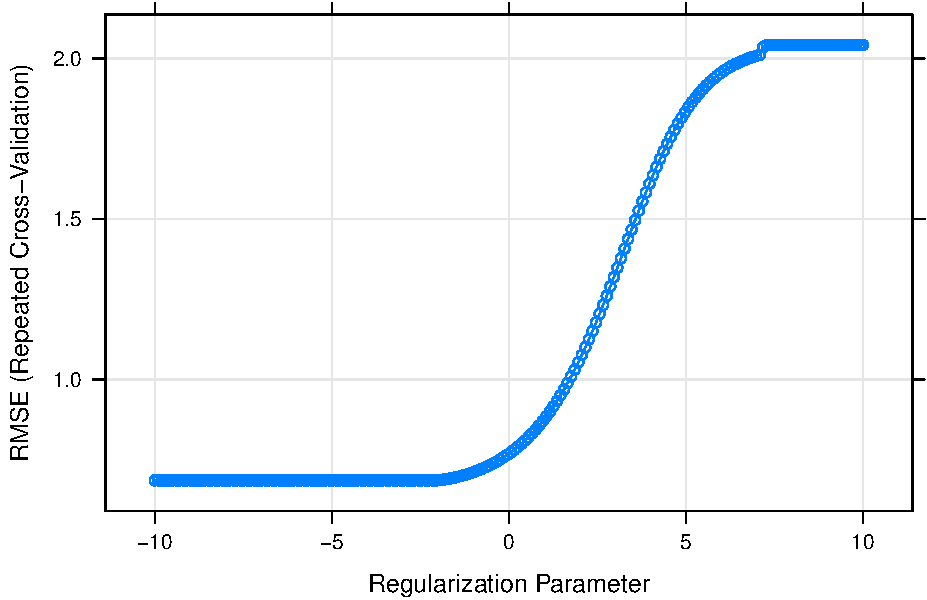
\includegraphics{P8106_Ec3342_Hw1_files/figure-latex/unnamed-chunk-5-1.pdf}

\begin{Shaded}
\begin{Highlighting}[]
\NormalTok{ridge.fit}\OperatorTok{$}\NormalTok{bestTune}
\end{Highlighting}
\end{Shaded}

\begin{verbatim}
##    alpha    lambda
## 80     0 0.1274155
\end{verbatim}

\begin{Shaded}
\begin{Highlighting}[]
\NormalTok{best_lambda <-}\StringTok{ }\NormalTok{ridge.fit}\OperatorTok{$}\NormalTok{bestTune}\OperatorTok{$}\NormalTok{lambda}
\NormalTok{best_lambda}
\end{Highlighting}
\end{Shaded}

\begin{verbatim}
## [1] 0.1274155
\end{verbatim}

\begin{Shaded}
\begin{Highlighting}[]
\NormalTok{ridge.pred =}\StringTok{ }\KeywordTok{predict}\NormalTok{(ridge.fit}\OperatorTok{$}\NormalTok{finalModel, }\DataTypeTok{s =}\NormalTok{ best_lambda, }\DataTypeTok{newx =}\NormalTok{ x_test) }
\CommentTok{#Using best lambda to predict test data}
\KeywordTok{mse}\NormalTok{(y_test, ridge.pred)}
\end{Highlighting}
\end{Shaded}

\begin{verbatim}
## [1] 0.5134603
\end{verbatim}

◆ The test error is 0.5134603.

\begin{enumerate}
\def\labelenumi{\alph{enumi})}
\setcounter{enumi}{2}
\tightlist
\item
  Fit a lasso model on the training data, with λ chosen by
  cross-validation. Report the test error, along with the number of
  non-zero coefficient estimates.
\end{enumerate}

\begin{Shaded}
\begin{Highlighting}[]
\KeywordTok{set.seed}\NormalTok{(}\DecValTok{2}\NormalTok{)}
\NormalTok{lasso.fit <-}\StringTok{ }\KeywordTok{train}\NormalTok{(x_train, y_train,}
                   \DataTypeTok{method =} \StringTok{"glmnet"}\NormalTok{,}
                   \DataTypeTok{tuneGrid =} \KeywordTok{expand.grid}\NormalTok{(}\DataTypeTok{alpha =} \DecValTok{1}\NormalTok{, }
                                          \DataTypeTok{lambda =} \KeywordTok{exp}\NormalTok{(}\KeywordTok{seq}\NormalTok{(}\OperatorTok{-}\DecValTok{10}\NormalTok{, }\DecValTok{10}\NormalTok{, }\DataTypeTok{length =} \DecValTok{200}\NormalTok{))),}
                   \CommentTok{# preProc = c("center", "scale"),}
                   \DataTypeTok{trControl =}\NormalTok{ ctrl1)}

\KeywordTok{plot}\NormalTok{(lasso.fit, }\DataTypeTok{xTrans =} \ControlFlowTok{function}\NormalTok{(x) }\KeywordTok{log}\NormalTok{(x))}
\end{Highlighting}
\end{Shaded}

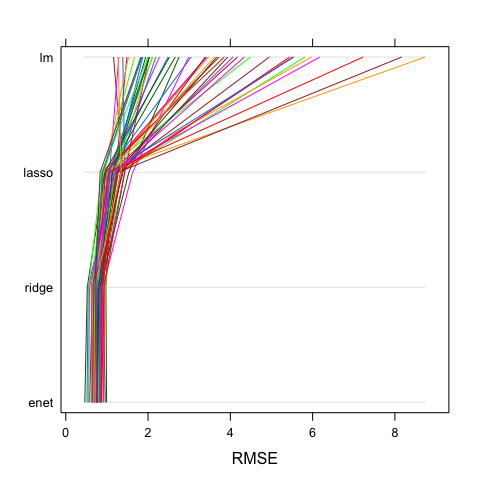
\includegraphics{P8106_Ec3342_Hw1_files/figure-latex/unnamed-chunk-8-1.pdf}

\begin{Shaded}
\begin{Highlighting}[]
\NormalTok{best_lambda_lasso <-}\StringTok{ }\NormalTok{lasso.fit}\OperatorTok{$}\NormalTok{bestTune}\OperatorTok{$}\NormalTok{lambda}
\NormalTok{best_lambda_lasso}
\end{Highlighting}
\end{Shaded}

\begin{verbatim}
## [1] 0.0046222
\end{verbatim}

\begin{Shaded}
\begin{Highlighting}[]
\NormalTok{lasso.pred =}\StringTok{ }\KeywordTok{predict}\NormalTok{(lasso.fit}\OperatorTok{$}\NormalTok{finalModel, }\DataTypeTok{s =}\NormalTok{ best_lambda_lasso, }\DataTypeTok{newx =}\NormalTok{ x_test) }
\CommentTok{#Using best lambda to predict test data}
\KeywordTok{mse}\NormalTok{(y_test, lasso.pred)}
\end{Highlighting}
\end{Shaded}

\begin{verbatim}
## [1] 0.4987333
\end{verbatim}

◆ The test error is 0.4987333

\begin{Shaded}
\begin{Highlighting}[]
\NormalTok{lasso.coef <-}\StringTok{ }\KeywordTok{coef}\NormalTok{(lasso.fit}\OperatorTok{$}\NormalTok{finalModel,lasso.fit}\OperatorTok{$}\NormalTok{bestTune}\OperatorTok{$}\NormalTok{lambda)}
\KeywordTok{length}\NormalTok{(lasso.coef)}
\end{Highlighting}
\end{Shaded}

\begin{verbatim}
## [1] 229
\end{verbatim}

\begin{Shaded}
\begin{Highlighting}[]
\KeywordTok{length}\NormalTok{(lasso.coef[lasso.coef }\OperatorTok{!=}\StringTok{ }\DecValTok{0}\NormalTok{])}
\end{Highlighting}
\end{Shaded}

\begin{verbatim}
## [1] 144
\end{verbatim}

◆ There are 144 non-zero coefficient estimates.

\begin{enumerate}
\def\labelenumi{\alph{enumi})}
\setcounter{enumi}{3}
\tightlist
\item
  Fit a principle component regression model on the training data, with
  M chosen by cross-validation. Report the test error, along with the
  value of M selected by cross-validation.
\end{enumerate}

\begin{Shaded}
\begin{Highlighting}[]
\KeywordTok{set.seed}\NormalTok{(}\DecValTok{2}\NormalTok{)}
\NormalTok{pcr.fit <-}\StringTok{ }\KeywordTok{train}\NormalTok{(x_train, y_train,}
                  \DataTypeTok{method =} \StringTok{"pcr"}\NormalTok{,}
                  \DataTypeTok{tuneLength =} \DecValTok{149}\NormalTok{,}
                  \DataTypeTok{trControl =}\NormalTok{ ctrl1,}
                  \DataTypeTok{scale =} \OtherTok{TRUE}\NormalTok{)}

\NormalTok{predy.pcr <-}\StringTok{ }\KeywordTok{predict}\NormalTok{(pcr.fit}\OperatorTok{$}\NormalTok{finalModel, }\DataTypeTok{newdata =}\NormalTok{ x_test, }
                       \DataTypeTok{ncomp =}\NormalTok{ pcr.fit}\OperatorTok{$}\NormalTok{bestTune}\OperatorTok{$}\NormalTok{ncomp)}
\KeywordTok{mse}\NormalTok{(y_test, predy.pcr)}
\end{Highlighting}
\end{Shaded}

\begin{verbatim}
## [1] 0.540555
\end{verbatim}

\begin{Shaded}
\begin{Highlighting}[]
\KeywordTok{ggplot}\NormalTok{(pcr.fit, }\DataTypeTok{highlight =} \OtherTok{TRUE}\NormalTok{) }\OperatorTok{+}\StringTok{ }\KeywordTok{theme_bw}\NormalTok{()}
\end{Highlighting}
\end{Shaded}

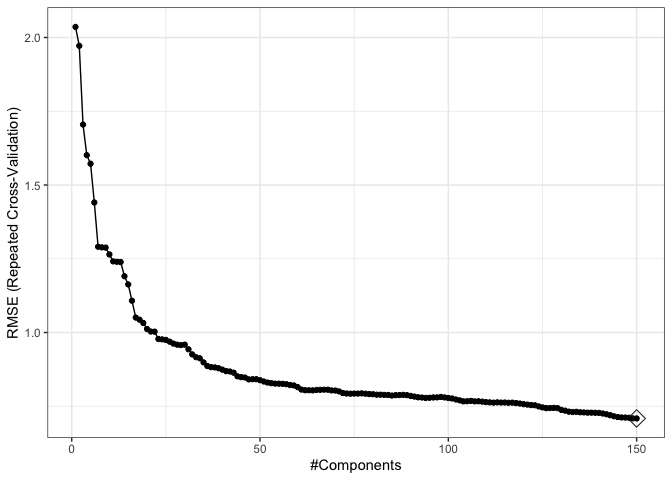
\includegraphics{P8106_Ec3342_Hw1_files/figure-latex/unnamed-chunk-12-1.pdf}
◆ The test error is 0.540555 ◆ The value of M selected by cross
validation is 149.

\begin{enumerate}
\def\labelenumi{\alph{enumi})}
\setcounter{enumi}{4}
\tightlist
\item
  Briefly discuss the results obtained in (a)∼(d).
\end{enumerate}

\begin{Shaded}
\begin{Highlighting}[]
\NormalTok{resamp <-}\StringTok{ }\KeywordTok{resamples}\NormalTok{(}\KeywordTok{list}\NormalTok{(}\DataTypeTok{lasso =}\NormalTok{ lasso.fit, }\DataTypeTok{ridge =}\NormalTok{ ridge.fit, }\DataTypeTok{pcr =}\NormalTok{ pcr.fit, }\DataTypeTok{lm =}\NormalTok{ lm.fit))}
\KeywordTok{summary}\NormalTok{(resamp)}
\end{Highlighting}
\end{Shaded}

\begin{verbatim}
## 
## Call:
## summary.resamples(object = resamp)
## 
## Models: lasso, ridge, pcr, lm 
## Number of resamples: 50 
## 
## MAE 
##            Min.   1st Qu.    Median      Mean   3rd Qu.      Max. NA's
## lasso 0.4252298 0.4840513 0.5177887 0.5173336 0.5484913 0.6385859    0
## ridge 0.4236514 0.4901614 0.5218728 0.5213242 0.5473545 0.6319687    0
## pcr   0.4324539 0.5072261 0.5466597 0.5426985 0.5809145 0.6606165    0
## lm    0.4151018 0.5042577 0.5288620 0.5304540 0.5607729 0.6838928    0
## 
## RMSE 
##            Min.   1st Qu.    Median      Mean   3rd Qu.      Max. NA's
## lasso 0.5582277 0.6414335 0.6701683 0.6775176 0.7145061 0.8331316    0
## ridge 0.5547163 0.6488957 0.6786781 0.6856755 0.7234002 0.8333606    0
## pcr   0.5640148 0.6711085 0.7188954 0.7091304 0.7449607 0.8618922    0
## lm    0.5763256 0.6702141 0.7006166 0.7093576 0.7470323 0.9234601    0
## 
## Rsquared 
##            Min.   1st Qu.    Median      Mean   3rd Qu.      Max. NA's
## lasso 0.8372380 0.8774330 0.8947011 0.8904805 0.9047275 0.9283355    0
## ridge 0.8326964 0.8764872 0.8908486 0.8880644 0.9001630 0.9264558    0
## pcr   0.8184227 0.8683917 0.8840107 0.8806591 0.8942654 0.9284906    0
## lm    0.8105782 0.8668429 0.8844072 0.8814378 0.8966132 0.9313096    0
\end{verbatim}

\begin{Shaded}
\begin{Highlighting}[]
\KeywordTok{bwplot}\NormalTok{(resamp, }\DataTypeTok{metric =} \StringTok{"RMSE"}\NormalTok{)}
\end{Highlighting}
\end{Shaded}

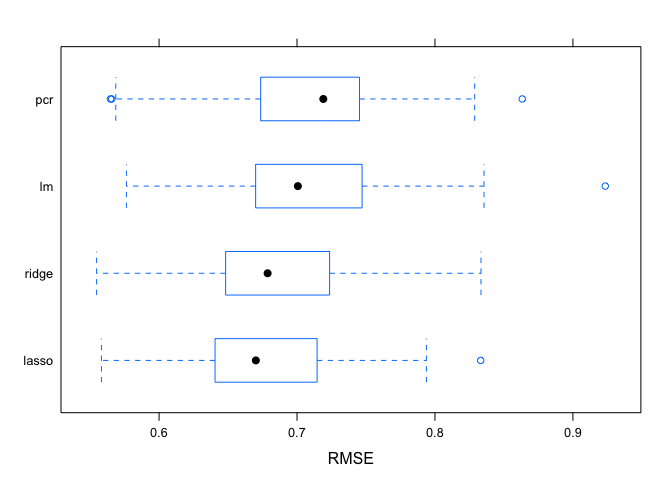
\includegraphics{P8106_Ec3342_Hw1_files/figure-latex/unnamed-chunk-13-1.pdf}

As we can see from the graph, the minimum RMSE is for Lasso followed by
Ridge model. The Linear model and the PCR has the maximum RMSE.

\begin{enumerate}
\def\labelenumi{\alph{enumi})}
\setcounter{enumi}{5}
\tightlist
\item
  Which model will you choose for predicting solubility?
\end{enumerate}

Since, the RMSE is the lowest for Lasso, we should choose the Lasso
model to predict solubility.


\end{document}
